\documentclass[12pt]{article}
\usepackage[T1]{fontenc}
%\usepackage[latin9]{inputenc}
\usepackage[utf8]{inputenc}
\usepackage[english]{babel}
\usepackage{amsmath}
\usepackage{amsfonts}
\usepackage{amssymb}
%\usepackage{setspace}
\usepackage{rotating}
\usepackage{graphics}
\usepackage{eurosym}
\usepackage[round]{natbib}
%\usepackage{graphicx}
%\usepackage{float} 				%allows you to float images
\usepackage{latexsym}
%\usepackage{bbding}
%\usepackage {moresize}
\usepackage{listings}
\usepackage{bbding}
\usepackage{blindtext}
\usepackage{hhline}
\usepackage{tikz}
\usetikzlibrary{trees}
%\usetikzlibrary{shapes,backgrounds}
%\usepackage{pgfplots}
%\usetikzlibrary{arrows}
\usepackage{enumitem}
%\doublespacing
%\usepackage{geometry}
\usepackage{amsthm}
\usepackage{color}
%\usepackage{array,multirow}
%\usepackage{subcaption}
%\usepackage{pst-plot}
%	\psset{xunit=15mm}
%\geometry{verbose,tmargin=1in,bmargin=1in,lmargin=.5in,rmargin=.5in}
\setlength{\parskip}{\bigskipamount}
\setlength{\parindent}{0pt}
\usepackage{multicol}

\newenvironment{problem}[3][Problem]{\begin{trivlist}
\item[\hskip \labelsep {\bfseries #1}\hskip \labelsep {\bfseries #2.}]}{\end{trivlist}}

\newcommand{\barr}{\bar{r}}
\newcommand{\ddx}{\frac{d}{dx}}
\newcommand{\infsum}{\sum_{n=1}^{\infty }}

\title{Problem Set 8 \thanks{Problems:5.2,5.4,5.6,5.7,5.12,5.16,5.17,5.20,5.27}}
\author{Ian McGroarty \\
	Course Number: 555.444 \\
}
\date{October, 21, 2019}

\begin{document}

\maketitle
\newpage
%%%%%%%%%%%%%%%%%%%%%%%%%%%%%%%%%%%%%%%%%%%%%%%%%%%%%%%%
%%%%%%%%%%%%%%%%%%%%%%%%%%%%%%%%%%%%%%%%%%%%%%%%%%%%%%%%
%%%%%%%%%%%%%%%%%%%%%%%%%%%%%%%%%%%%%%%%%%%%%%%%%%%%%%%%
\begin{problem}{11.7}. $S=19, K=20, c = 1, r=0.04. $
\begin{align*}
c + Ke^{-rT} &= p + S_0 && \text{Put-Call parity} \\
1 + 20e^{0.04*(3/12) }&= p + 19 \\
p &= 1.8 
\end{align*}
\end{problem}


\begin{problem}{11.14}. K=30, c=2, $S_0=29$ D=0.5, r=0.1, p = ?.
\begin{align*}
c+Ke^{-rT}+D &= p +S_0 && \text{Put Call Parity} \\
2 + 30 e^{0.1*(6/12)} + &0.5 e^{-0.1*(2/12)} + 0.5e^{-0.1 *(5/12)} - 29 = p \\
p &= 2.51
\end{align*}
\end{problem}

\begin{problem}{11.15}. So the price of the put would be overvalued so we can buy the call and short the stock and the put: This would give a positive upfront gain of $(3-2+29)= 30.$ When invested at the risk free rate this grows to $30e^{.1*3/12} = 30.76$. No matter what happens the investor will buy a stock for \$30 at time T and have a profit of \$0.76. 

\end{problem}

\newpage
\begin{problem}{11.18}. Based on the hint in the book, I\rq{}ll consider:
\begin{align*}
\text{Portfolio A:} & \text{One European Call and K in cash} \\
\text{Portfolio B:} & \text{One American Put and one share of the stock} \\
\end{align*}
The value of portfolio A at time T is: $max(S_T - K,0) + Ke^{rt} \rightarrow max(S_T,K)-K+Ke^{rt}$. The value of portfolio B at time T is a little more compliacted because of the posibility of early exercise. To see this first consider that for a similar portfolio with a european put instead, the value is $max(K-S_T,0) + S_T$ But since there is the posibility of early exercise you have to forward the profit from selling the put: $max([K-S_T]e^{r(T-t)},0) + S_T \rightarrow max(K,S_T)e^{r(T-t)} $ It is pretty clear from these two valuation to see that portfolio A is worth more than portfolio B. So.
\begin{align*}
c + K & \geq P + S_0 \\
c - P & \geq S_0 - K \\
 C - P & \geq S_0 - K  && \text{Since c=C pg 243} \\
\text{To continue we can use the put call parity} \\
c+Ke^{-rT}&=p + S_0 &&\text{Eqn. 11.6 pg 239} \\
c-p &= S_0 - Ke^{-rT} \\
C-p &= S_0 - Ke^{-rT} && \text{see above} \\
C-P &\leq S_0 - Ke^{-rT} && p \leq P \text{  pg 246} \\
 S_0 - K \leq C-P &\leq S_0 - Ke^{-rT}
\end{align*}
\end{problem}

\newpage
\begin{problem}{11.19}. Based on the hint from the book, I consider:
\begin{align*}
\text{Portfolio A:} & \text{One European Call and (K+D) in cash} \\
\text{Value A: } & max(S_T-K,0) + (K+D)e^{rT}  \rightarrow max(S_T,K) - K + (K+D)e^{rT} \\
\text{Portfolio B:} & \text{One American Put and one share of the stock} \\
\text{Value B:} & max(K-S_T,0)e^{r(T-t)} + S_T + De^{rT} \\ 
\end{align*}
This is similar to 11.18 so I won\rq{}t go into it as much. But similarly we can see the $A\geq B$ so 
\begin{align*}
c+K+D \geq P + S_0 \\
C-P \geq S_0 - K - D \\
\text{From the put call parity for options with dividends:} \\
c+D+Ke^{-rT} &= p + S_0 \\ 
C-P + D \leq S_0 - Ke^{-rT}
\end{align*}
Since dividends decrease C and increase P the result holds that $$C-P\leq S_0 - Ke^{-rT}$$
\end{problem}
\newpage

\begin{problem}{11.25}. With $K_1 < K_2 < K_3$ and $K_3 - K_2 = K_2 - K_1$. Using the hint from the book we consider 1 long call on $K_1$ and $K_3$ and 2 short calls on $K_2$. An example graph is shown below. 
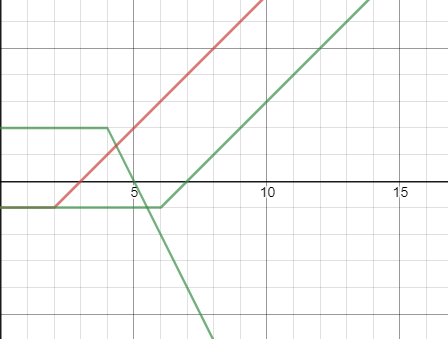
\includegraphics[width=.5\textwidth]{mod8p24.png}
From the figure we can see easy that $c_2 = 0.5(c_1 + c_3)$. So let us consider this. First note that $c_1 = max(S-K_1,0)$, and $c_2 = 2\cdot max(K_2-S,0)$, and finally, $c_3 = max(S-K_3,0)$. One quick way to see this is to put the three options in one portfolio and see that:
\begin{align*}
\text{Case 1:}& S \leq K_1 \implies \text{All worth 0} \\
\text{Case 2:}& K_1 < S \leq K_2 \implies c_1>0 \& c_2 = 0 \\
\text{Case 3:}& K_1 < K_2 \leq S < K_3 \implies (S-K_1) - 2(S-K_2) = 2K_2 -S - K \geq 0 \\
\text{Case 4:}& K_3 < S  \implies (S-K_1) -2(S-K_2) + (S-K_3) = 2K_2 - K_1 = K_3 \geq 0 \\
\text{Since:  }& c_1 -2c_2 + c_3 \geq 0 \implies 0.5(c_1 + c_3) \geq c_2
\end{align*}
\end{problem}







\end{document}